\documentclass{article}

\PassOptionsToPackage{numbers,compress}{natbib}
\usepackage[final]{neurips_2024}

\usepackage[utf8]{inputenc}
\usepackage[T1]{fontenc}
\usepackage{amsmath}
\usepackage{amsfonts}
\usepackage{booktabs}
\usepackage{float}
\usepackage{graphicx}
\usepackage{microtype}
\usepackage[section]{placeins}
\usepackage{url}
\usepackage{xcolor}

\makeatletter
\renewcommand{\@notice}{}
\makeatother

\setlength{\textfloatsep}{9pt plus 2pt minus 2pt}
\setlength{\floatsep}{9pt plus 2pt minus 2pt}
\setlength{\intextsep}{8pt plus 2pt minus 2pt}
\setlength{\abovecaptionskip}{5pt}
\setlength{\belowcaptionskip}{4pt}
\newcommand{\ppr}{\mathrm{PPR}}
\newcommand{\good}[1]{\textcolor{green!40!black}{\textbf{#1}}}
\newcommand{\bad}[1]{\textcolor{red!65!black}{#1}}

\title{Expected Points Are Not Enough: Modeling Weekly Fantasy Football Projections and Boom-Game Risk}

\author{%
  Umair Siddiqui (NetID uss12) \quad
  Yash Singh (NetID ys1008) \quad
  Section ID: TODO
}

\begin{document}

\maketitle

\begin{abstract}
Weekly fantasy football projection is usually treated as expected-value regression, but lineup decisions also depend on upside: rare high-ceiling games that conditional-mean models smooth away. Using NFL player-week data from 2017--2024, we train on 2018--2022, tune on 2023, and test only on 2024, with 2017 used solely as prior history. Our enhanced LightGBM expected-point model improves RMSE from 6.25 to 6.06 and MAE from 4.67 to 4.49; paired player-cluster bootstrap intervals support both gains. In a contextual comparison to published IBM/ESPN fantasy projection metrics, our model outperforms the reported values with lower RMSE (6.06 vs. 6.78) and higher within-10/within-7 rates (90.7\%/80.2\% vs. 88.2\%/71.0\%), with the advantage preserved in a top-500 sensitivity analysis. The expected model still underpredicts 99.4\% of 20+ point games. A p90 quantile model reduces high-score MAE from 11.59 to 5.38, showing that expected value and ceiling are distinct forecasting objects. We therefore pair expected-point regression with calibrated boom classifiers at 10, 15, and 20 PPR thresholds. Code: \url{[public GitHub link]}
Video: \url{[public video link]}
\end{abstract}
\enlargethispage{4\baselineskip}

\section{Introduction}
Fantasy football is a weekly forecasting problem with unusually visible consequences. A manager does not only ask whether a player is good in expectation; they ask whether a player is likely to beat a replacement option this week, whether a matchup creates enough upside to justify risk, and whether a low-floor option should be avoided. This makes the task a natural data science setting: every game creates labeled feedback, the features have temporal structure, the target distribution is skewed, and the decision problem is sensitive to both average error and tail behavior.

The central question of this project is whether historical NFL player-week statistics can support two complementary forecasts: (i) a regression forecast of weekly PPR fantasy points and (ii) a classification forecast of whether a player will exceed boom thresholds of 10, 15, and 20 PPR points. The first task estimates expected value. The second asks whether the model can identify high-ceiling outcomes, especially for players whose mean projection is modest but whose role, matchup, or prior volatility leaves room for an outsized week.

Our main finding is that the two tasks expose different strengths and failures. The enhanced expected-point model is a better average forecaster than the original pipeline: on the 2024 test season, RMSE improves from 6.25 to 6.06 and $R^2$ improves from 0.401 to 0.437. Yet expected-point regression remains strongly conservative in the tail. Among 545 player-weeks with at least 20 PPR points, the enhanced model has 11.59 MAE and predicts below the actual value in 99.4\% of cases. Quantile regression reverses part of this failure: the p90 model reduces 20+ point MAE to 5.38, but it overprojects lower-scoring players and raises overall RMSE to 9.39. This is not a bug in the quantile model; it is evidence that ceiling projection is a different target than expected points.

We make three contributions. First, we build a leakage-safe temporal modeling pipeline for weekly fantasy projections across QB, RB, and WR/TE groups. Second, we evaluate feature additions through controlled ablations, including recent form, prior-season production, defensive matchup features, player career profiles, temporal features, and team opportunity-share features. Third, we report both expected-value metrics and boom-classification metrics, making the expected-value/upside tradeoff explicit rather than hiding it behind a single point-projection score.

\section{Related Work}
Fantasy football has been studied both as a prediction problem and as a downstream optimization problem. Lutz \citep{lutz2015fantasy} studied quarterback score prediction with support vector regression and neural networks, emphasizing the difficulty of limited structured data. Landers and Duperrouzel \citep{landers2019machine} used machine learning to predict NFL fantasy points and then construct lineups for daily fantasy contests. Matthews, Ramchurn, and Chalkiadakis \citep{matthews2012competing} considered automated team formation against human fantasy managers in a partially observable setting, while Mahoney and Paniak \citep{mahoney2023method} combined machine learning projections with linear programming for daily fantasy lineup optimization. These works motivate fantasy football as a domain where predictive quality matters because forecasts become roster decisions.

The closest contextual comparison is the IBM/ESPN system of Baughman et al. \citep{baughman2021deep}, which combined structured ESPN data, injury reports, and large-scale language understanding over news, articles, audio, and video. Their system classified player states such as boom, bust, hidden injury, and meaningful touches, then fed those signals into a regression ensemble. They report 6.78 RMSE for top 500+ players, 88.2\% of projections within 10 points, and 71\% within 7 points. Our enhanced expected model reports 6.06 RMSE, 90.7\% within 10 points, and 80.2\% within 7 points. This should be read only as a contextual comparison: seasons, scoring populations, expert projections, injury/news inputs, and player inclusion criteria differ substantially.

Methodologically, our strongest point-projection models use LightGBM \citep{ke2017lightgbm}, a gradient-boosted decision tree method well suited to tabular data with nonlinear feature interactions. To model ceiling rather than only conditional mean, we use quantile regression ideas introduced by Koenker and Bassett \citep{koenker1978regression}. For boom classification, class imbalance makes accuracy insufficient; precision, recall, F1, ROC-AUC, and average precision better expose the tradeoff between missed boom games and false alarms \citep{davis2006relationship}. We also test isotonic calibration, following the broader observation that probability estimates from supervised learners often need post-hoc calibration \citep{niculescu2005predicting}.

\section{Data}
The project uses three canonical Supabase tables, one per position group: \texttt{QBPointProjection}, \texttt{RBPointProjection}, and \texttt{WRTEPointProjection}. The tables contain 4,857 QB rows, 11,668 RB rows, and 28,205 WR/TE rows across the 2017--2024 NFL seasons. Each row is a structured player-week record with identifiers, team and opponent, season and week, PPR fantasy points, lagged player statistics, rolling player statistics, prior-season summaries, and opponent defensive allowed features. The modeling scripts restrict weeks to the regular fantasy-relevant range and train separate models by position group because QB, RB, and WR/TE usage distributions differ.

We use a temporal split rather than a random split. The 2017 season is not part of the supervised training set; it is used only as legitimate prior history when constructing enhanced features for early 2018 observations. Training uses 2018--2022, validation and threshold selection use 2023, and the final test set is the 2024 season. This matches the real forecasting setting: future weeks and future seasons are unavailable when a weekly projection is made.

\begin{figure}[!htbp]
  \centering
  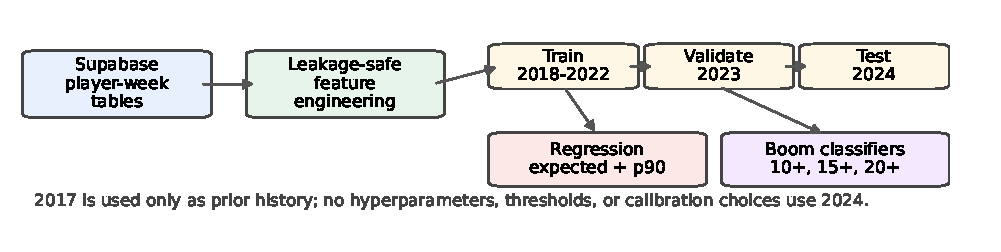
\includegraphics[width=0.98\linewidth]{figures/pipeline_temporal_split.pdf}
  \caption{End-to-end modeling protocol. Supabase player-week tables feed leakage-safe historical features; training, tuning, and testing are separated by season.}
  \label{fig:pipeline}
\end{figure}

\begin{table}[!htbp]
\caption{Dataset summary by position group. Table row counts are the verified Supabase counts for 2017--2024; the held-out summaries are computed from active 2024 result artifacts. The 2017 season is retained only as pre-2018 history for leakage-safe features; model training uses 2018--2022, validation uses 2023, and the reported test set is 2024.}
\label{tab:dataset}
\centering
\footnotesize
\begin{tabular}{lrrrrr}
\toprule
Pos. & Table rows & 2024 rows & 2024 players & 2024 mean & 2024 20+ \\
\midrule
QB & 4,857 & 643 & 72 & 14.17 & 25.3\% \\
RB & 11,668 & 1,452 & 124 & 8.14 & 9.5\% \\
WR/TE & 28,205 & 3,660 & 362 & 6.79 & 6.7\% \\
\bottomrule
\end{tabular}
\end{table}


Table~\ref{tab:dataset} also foreshadows the modeling difficulty. Most player-weeks are low or moderate scoring, but the right tail is strategically important. The 20+ threshold is common for quarterbacks, rarer for running backs, and rarest for WR/TE, where it represents a sparse high-upside event.

\section{Feature Engineering}
The feature pipeline is designed around information that would be known before kickoff. We exclude the current week's target and remove the direct previous fantasy-points column from the feature matrix when it would duplicate engineered history. Missing early-season values are handled by the estimators or by median imputation in linear/logistic baselines.

\begin{table}[!htbp]
\caption{Feature groups used in the projection system.}
\label{tab:features}
\centering
\footnotesize
\begin{tabular}{p{0.25\linewidth}p{0.67\linewidth}}
\toprule
Group & Examples and purpose \\
\midrule
Recent player form & One-week lags and rolling 3/5-week means for passing, rushing, receiving, and fantasy output. These capture current role and short-term usage. \\
Prior-season context & Previous-season games, volume, yardage, touchdowns, and per-game rates. These stabilize early-season projections when current-season history is sparse. \\
Defensive matchup & Rolling opponent points and box-score production allowed to the relevant position group. These encode matchup strength without using future games. \\
Enhanced profile & Prior career mean, standard deviation, p75, p90, max, prior boom rates, season-to-date mean, and temporal week indicators. These target player ceiling and volatility. \\
Opportunity share & Player share of team/position rolling attempts, carries, targets, receptions, and yardage. These distinguish a player's own workload from team environment. \\
\bottomrule
\end{tabular}
\end{table}

The original aligned experiments compare rolling-only features, rolling plus prior-season features, full features without defensive allowed variables, and full features. The enhanced experiments add career profile, temporal, season-to-date, prior boom-rate, and team opportunity-share features. Because all rolling, career, and season-to-date quantities are shifted before the current observation, the enhanced features can use 2017 as history without leaking 2018--2024 outcomes.

\section{Method}
\paragraph{Regression models.}
For each position group we train a linear regression baseline and several LightGBM regressors. The primary model is an expected-points LightGBM regressor tuned on 2023 validation RMSE. The original pipeline uses a fixed LightGBM configuration; the enhanced pipeline selects over tree complexity, minimum child samples, regularization, and feature subsampling. We also train a boom-weighted LightGBM model that upweights high-scoring training examples, and quantile LightGBM models at p50, p75, and p90. The quantile models optimize asymmetric loss and should be interpreted as median or ceiling projections rather than expected values.

\paragraph{Boom classification models.}
For each position group and threshold $\tau \in \{10,15,20\}$, the binary label is
\[
  y_{i,\tau} = \mathbb{1}[\mathrm{fantasy\_points\_ppr}_i \geq \tau].
\]
We evaluate majority-class baselines, logistic regression, class-balanced logistic regression, default LightGBM, class-balanced LightGBM, validation-threshold-tuned LightGBM, and enhanced variants. For enhanced classifiers, we also fit isotonic calibration on the 2023 validation probabilities and then choose the F1-maximizing decision threshold on 2023. This avoids selecting thresholds on the 2024 test set.

\paragraph{Overfitting controls and evaluation protocol.}
We control overfitting and underfitting through a held-out temporal validation year, LightGBM early stopping, regularization and minimum-leaf-size candidates in the enhanced search, ablations against lower-complexity feature sets, and linear/logistic baselines. No hyperparameters, thresholds, or calibration choices are selected on the 2024 test season. Regression is evaluated with MAE, RMSE, $R^2$, bias, within-7 and within-10 point rates, and high-score metrics on the subset with at least 20 PPR points. Classification is evaluated with accuracy, precision, recall, F1, ROC-AUC, average precision, Brier score, actual positive rate, and predicted positive rate. We emphasize F1 and average precision for boom prediction because the rare thresholds, especially WR/TE 20+, are imbalanced.

\section{Evaluation}
\subsection{Regression Results}
Table~\ref{tab:regression-overall} summarizes the overall expected-point results on the 2024 test set. The enhanced LightGBM expected model improves every main average-error metric: MAE falls from 4.67 to 4.49, RMSE from 6.25 to 6.06, and $R^2$ rises from 0.401 to 0.437. The within-10 rate increases from 90.3\% to 90.7\%, and the within-7 rate increases from 79.8\% to 80.2\%. The improvement is modest but consistent, which is a useful result in a noisy weekly sports domain.

A paired player-cluster bootstrap confirms that the average-error gains are robust: RMSE reduction is 0.19 [0.13, 0.25], and MAE reduction is 0.18 [0.13, 0.23].


\begin{table}[!htbp]
\caption{Overall held-out 2024 point-projection performance across all positions.}
\label{tab:regression-overall}
\centering
\footnotesize
\begin{tabular}{lrrrrrr}
\toprule
Model & MAE & RMSE & $R^2$ & $|e|\leq7$ & $|e|\leq10$ & 20+ MAE \\
\midrule
Original LightGBM expected & 4.67 & 6.25 & 0.401 & 79.8\% & 90.3\% & 12.04 \\
Enhanced LightGBM expected & 4.49 & 6.06 & 0.437 & 80.2\% & 90.7\% & 11.59 \\
\bottomrule
\end{tabular}
\end{table}


Table~\ref{tab:regression-position} breaks the expected model down by position. Quarterbacks have the largest absolute RMSE because their scoring range is wider, but they also benefit the most from enhanced features. RB and WR/TE improvements are smaller in RMSE terms, partly because their score distributions contain many low-volume observations near zero.

\begin{table}[!htbp]
\caption{Expected-point regression results by position group on the 2024 test season.}
\label{tab:regression-position}
\centering
\footnotesize
\begin{tabular}{lrrrrrr}
\toprule
Pos. & Rows & Orig. RMSE & Enh. RMSE & $\Delta$ & Enh. MAE & Enh. 20+ MAE \\
\midrule
QB & 643 & 8.05 & 7.44 & 0.61 & 5.96 & 9.20 \\
RB & 1,452 & 6.22 & 6.00 & 0.22 & 4.47 & 11.80 \\
WR/TE & 3,660 & 5.89 & 5.80 & 0.09 & 4.24 & 13.06 \\
\bottomrule
\end{tabular}
\end{table}


This position-level pattern is important for interpreting the overall score. The test set is dominated by WR/TE player-weeks, so an aggregate RMSE can look strong while still masking quarterback volatility or rare receiver ceiling. For that reason we do not select models only by the pooled metric. Validation is performed by position group, and the final reporting includes both pooled and position-specific views.

\subsection{Feature Ablations}
Table~\ref{tab:ablation} reports the original LightGBM ablation. Rolling recent-form features already provide a strong baseline. Prior-season production improves all three position groups, especially RB and WR/TE. Defensive matchup features help RB and WR/TE slightly but do not help QB in this pass; this is plausible because quarterback scoring depends heavily on game script, rushing production, and team-level passing environment, not only what a defense has recently allowed.

\begin{table}[!htbp]
\caption{Original LightGBM feature ablation on the 2024 test season.}
\label{tab:ablation}
\centering
\footnotesize
\begin{tabular}{lrrrr}
\toprule
Feature set & Max feats. & QB RMSE & RB RMSE & WR/TE RMSE \\
\midrule
Rolling only & 36 & 8.07 & 6.45 & 6.05 \\
+ Previous season & 49 & 7.94 & 6.27 & 5.90 \\
Full minus defense & 49 & 7.96 & 6.27 & 5.90 \\
+ Defensive matchup & 59 & 8.05 & 6.22 & 5.89 \\
\bottomrule
\end{tabular}
\end{table}


The enhanced model improves over this original feature set by adding player profile and opportunity-share signals. These additions are most valuable when a raw rolling mean is ambiguous: a player can have the same recent fantasy average with a different target share, team opportunity total, prior boom history, or career ceiling.

The ablation also illustrates the model-complexity tradeoff. Adding features is useful only when those features encode stable pregame information. Defensive features add many matchup columns, but their benefit is position-dependent and not monotone. Enhanced profile features increase dimensionality further, so the tuned LightGBM search uses smaller leaf counts and regularization candidates to avoid simply memorizing recent outliers. The validation year is therefore not a formality; it is the guardrail that decides whether extra flexibility improves generalization.

\begin{table}[!htbp]
\caption{Top enhanced expected-model LightGBM features by gain on the training/validation fit. Percentages are normalized within each position model.}
\label{tab:importance}
\centering
\footnotesize
\begin{tabular}{lp{0.76\linewidth}}
\toprule
Pos. & Top gain-based features \\
\midrule
QB & player fp\_roll8\_mean (11.1\%); team share\_completions\_roll3 mean (10.0\%); team share\_attempts\_roll5 mean (8.1\%); team share\_completions\_roll5 mean (7.7\%); team total\_attempts\_roll3 mean (6.7\%) \\
RB & team share\_rushing\_yards\_roll5 mean (21.0\%); player fp\_roll8\_mean (18.2\%); team share\_rushing\_yards\_roll3 mean (12.7\%); player fp\_roll5 mean (7.9\%); team share\_carries\_lag1 (4.3\%) \\
WR/TE & player fp\_roll8\_mean (45.7\%); player fp\_career\_mean\_prior (17.1\%); team share\_targets\_roll5 mean (6.2\%); player fp\_career\_p75\_prior (4.0\%); player fp\_roll5 mean (2.3\%) \\
\bottomrule
\end{tabular}
\end{table}


\subsection{Tail Risk and Quantile Models}
The most important failure mode is not average error but tail underprediction. The enhanced expected model has 11.59 MAE on 20+ point games and underpredicts 99.4\% of them. This is an expected consequence of conditional-mean regression under a skewed outcome distribution: the model is rewarded for staying near the dense center of the distribution, not for chasing rare ceiling outcomes.

\begin{table}[!htbp]
\caption{Tail-risk comparison on 2024. Quantile models are useful as ceiling estimates, but they are not replacements for calibrated expected-point projections.}
\label{tab:tail}
\centering
\footnotesize
\begin{tabular}{lrrrrr}
\toprule
Model & MAE & RMSE & 20+ MAE & 20+ under & $|e|\leq10$ \\
\midrule
Expected & 4.49 & 6.06 & 11.59 & 99.4\% & 90.7\% \\
Boom-weighted & 4.74 & 6.24 & 10.21 & 97.4\% & 89.3\% \\
Quantile p75 & 5.31 & 6.70 & 8.39 & 92.7\% & 86.8\% \\
Quantile p90 & 8.14 & 9.39 & 5.38 & 71.0\% & 68.8\% \\
Expected/p90 blend & 8.11 & 9.35 & 5.39 & 72.3\% & 69.1\% \\
\bottomrule
\end{tabular}
\end{table}


Table~\ref{tab:tail} shows that the p90 quantile model behaves like an upside model. It lowers 20+ point MAE to 5.38 and reduces the high-score underprediction rate to 71.0\%. However, the price is severe: overall RMSE worsens to 9.39 and only 68.8\% of predictions fall within 10 points. Figure~\ref{fig:tail} visualizes the same pattern. The expected model is accurate around the middle of the distribution but becomes increasingly negative in the tail. The p90 model stays closer to high-score outcomes but overpredicts low and mid-range games. Therefore, the p90 model should not replace the expected projection. It is better framed as a ceiling estimate that complements the expected-value forecast.

\begin{figure}[!htbp]
  \centering
  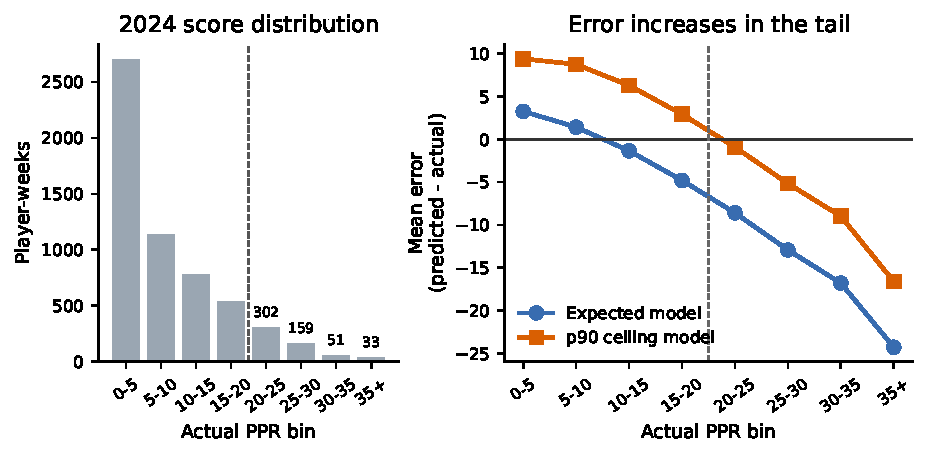
\includegraphics[width=0.98\linewidth]{figures/tail_residuals.pdf}
  \caption{Score distribution and mean residual by actual scoring bin. High-score outcomes are sparse, but the expected model's underprediction grows sharply in this tail. The p90 model reduces tail error while overpredicting lower-score bins.}
  \label{fig:tail}
\end{figure}
\FloatBarrier

\subsection{Boom Classification}
Figure~\ref{fig:boom-heatmap} summarizes the boom-classification results. Enhanced features improve five of the nine F1 tasks clearly and tie or nearly tie WR/TE 15+. The largest gains are QB 10+ (0.833 to 0.855), QB 15+ (0.656 to 0.681), RB 10+ (0.695 to 0.711), and RB 15+ (0.535 to 0.561). The 20+ tasks are harder because the positive class is smaller and more dependent on rare touchdowns, long plays, and game environment. RB 20+ is slightly worse after enhancement, and WR/TE 20+ drops from 0.339 to 0.302 despite similar ROC-AUC and average precision, suggesting that thresholded high-end receiver outcomes remain poorly captured by structured historical data alone.

\begin{figure}[!htbp]
  \centering
  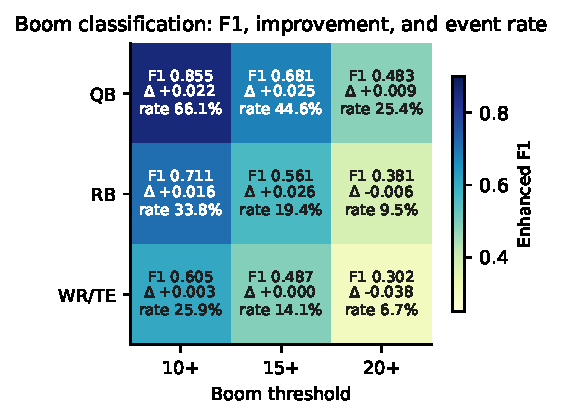
\includegraphics[width=0.78\linewidth]{figures/boom_classification_heatmap.pdf}
  \caption{Boom-classification summary. Cell color is enhanced F1; text reports enhanced F1, F1 change from the best original baseline, and the 2024 positive rate.}
  \label{fig:boom-heatmap}
\end{figure}

The enhanced classifiers often choose low decision thresholds and high recall, especially for QB thresholds. This is reasonable for a boom-screening task: users may prefer a shortlist of candidates with high recall, then combine the probability with expected points, risk tolerance, and roster context. Still, the low precision at 20+ thresholds shows that boom classification should be interpreted probabilistically, not as a deterministic start/sit rule.

Calibration is useful but not a cure-all. Figure~\ref{fig:calibration} shows that higher predicted probabilities generally correspond to higher observed boom rates, especially for 10+ and 15+ events, but F1 still depends on the final decision threshold and the base rate of the event.

\begin{figure}[!htbp]
  \centering
  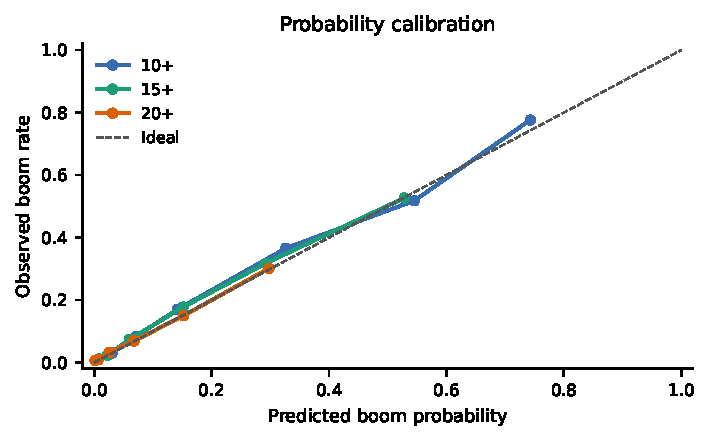
\includegraphics[width=0.68\linewidth]{figures/boom_probability_calibration.pdf}
  \caption{Reliability plot for isotonic-calibrated boom probabilities. Predictions are grouped into equal-frequency bins within each threshold and compared with observed boom rates; the diagonal is perfect calibration.}
  \label{fig:calibration}
\end{figure}

The WR/TE 20+ task has only 244 positives among 3,660 WR/TE test player-weeks, or 6.7\% of the WR/TE test set and 4.2\% of all 2024 test rows. This is an important tail failure to report, but it is also a fringe slice of the data distribution rather than the behavior of the overall projection system. Even a ranking model with reasonable ROC-AUC can have a low F1 once such a rare event is converted into binary predictions. This is why we report average precision and Brier score in the result artifacts while using Figure~\ref{fig:boom-heatmap} as the compact paper summary.

\subsection{Contextual Comparison to Prior Work}
Baughman et al. \citep{baughman2021deep} report 6.78 RMSE for their combined IBM/ESPN projection system over top 500+ fantasy players, with 88.2\% of projections within 10 points and 71\% within 7 points. Table~\ref{tab:espn-comparison} compares those published point estimates to our enhanced expected model on both the full 2024 test set and a top-500 sensitivity slice ranked by 2024 total PPR. To gauge uncertainty, we bootstrap our test metrics by resampling players with replacement; all three IBM/ESPN point estimates fall outside the worse side of our 95\% intervals in both scopes. This gives the comparison more weight than point estimates alone, but it is still not a direct benchmark because IBM/ESPN raw predictions are unavailable and the evaluation seasons, player inclusion rules, and input features differ.

\begin{table}[!htbp]
\caption{Contextual comparison to published IBM/ESPN point-projection metrics. Green indicates the better value. Confidence intervals are player-cluster bootstrap intervals for our 2024 test set; the top-500 slice ranks players by 2024 total PPR points to better match the published top-500+ population.}
\label{tab:espn-comparison}
\centering
\footnotesize
\begin{tabular}{llrrr}
\toprule
Metric & Better & IBM/ESPN & All 2024 (95\% CI) & Top-500 (95\% CI) \\
\midrule
RMSE & Lower & \bad{6.78} & \good{6.06} [5.82, 6.29] & \good{6.13} [5.88, 6.37] \\
Within 10 pts & Higher & \bad{88.2\%} & \good{90.7\%} [89.6, 91.7]\% & \good{90.4\%} [89.3, 91.5]\% \\
Within 7 pts & Higher & \bad{71.0\%} & \good{80.2\%} [78.6, 81.8]\% & \good{79.6\%} [77.9, 81.3]\% \\
\bottomrule
\end{tabular}
\end{table}

\FloatBarrier

\subsection{Qualitative Error Analysis}
The largest residuals are intuitive football events: extreme multi-touchdown games, sudden target spikes, and star players whose ceiling is much higher than their median week. In the enhanced 2024 predictions, Ja'Marr Chase's 55.4 point Week 10 is projected at 21.5 by the expected model and 29.0 by the p90 model. Josh Allen's 51.9 point Week 14 is projected at 21.8 expected and 29.2 p90. Jauan Jennings' 46.5 point Week 3 is projected at 8.2 expected and 19.3 p90. Quantile modeling moves in the right direction, but even p90 does not fully anticipate the most extreme weeks. Conversely, the quantile model overprojects low-score games because it is deliberately estimating a high conditional quantile. These examples reinforce the need to expose both expected and ceiling outputs.

The opposite error pattern also matters: established stars can be overprojected into quiet weeks when lagged usage cannot see injuries, blowouts, defensive adjustments, or sudden role changes. These misses point toward missing covariates such as injury reports, depth charts, betting totals, and text signals similar in spirit to the IBM/ESPN system.

\FloatBarrier
\section{Discussion}
The main lesson is that weekly fantasy football projection is multi-objective. If the goal is stable expected value, the enhanced LightGBM expected model is the best primary forecast. It improves average error, keeps most predictions within a usable range, and remains reasonably calibrated for ordinary weeks. If the goal is upside detection, the p90 quantile model and boom classifiers are more informative, but they should be consumed as risk signals rather than point estimates.

The feature results also show that domain-specific aggregation matters. Rolling box-score statistics capture immediate usage, but they are not enough to identify ceiling. Prior boom rates, career p90, opportunity share, and season-to-date form add information about a player's role and volatility. Defensive allowed features help for some positions but are not uniformly beneficial, which cautions against treating matchup labels as universally reliable. A strong fantasy system should therefore separate player talent/history, current role, team opportunity, and opponent context instead of collapsing them into a single average projection.

For practical fantasy decisions, the outputs are complementary. A manager choosing between safe options might prioritize expected points, while a manager projected to lose by a large margin might prefer a lower-mean player with a higher p90 or boom probability. The system does not directly optimize lineups, but its outputs can feed the downstream lineup and roster optimization studied in prior fantasy work.

\section{Limitations}
The model uses structured player-week statistics but omits several signals that fantasy managers rely on: explicit injury reports, depth charts, betting lines, weather, expert projections, snap-count forecasts, practice participation, and unstructured news/media. These omissions matter most for sudden role changes, such as backup running backs after an injury, receivers promoted by depth-chart changes, quarterbacks returning from injury, or games affected by weather and game script.

The boom labels are threshold-based rather than utility-based. A 20+ point game has different meaning for QB than WR/TE because base rates differ, and a useful fantasy decision may depend on replacement level, league size, roster slot, and opponent context. The classification models also optimize F1 on 2023, which is reasonable for controlled evaluation but not necessarily aligned with every fantasy user's cost function. Finally, WR/TE 20+ games remain hard. They are rare, often driven by long touchdowns or concentrated targets, and may require route-level, injury, defensive coverage, or betting-market features that are not present here.

\section{Conclusion}
This project builds a weekly fantasy football projection system on NFL player-week data from 2017--2024. The enhanced expected-point model improves 2024 regression performance and compares favorably to published IBM/ESPN projection metrics, but tail analysis shows that expected points alone hide high-ceiling risk. Quantile regression and boom classification make the final system a two-output forecaster: expected value plus upside probability or ceiling.

\clearpage
\bibliographystyle{plainnat}
\bibliography{references}

\end{document}
